\documentclass[fypca]{socreport}

\usepackage{fullpage}
\usepackage{graphicx}
\usepackage{enumitem}
\graphicspath{{./figs/}}

%%% Begin document
\begin{document}
\pagenumbering{roman}
\title{Underwater Real-Time Object Recognition and Tracking for Autonomous Underwater Vehicle}
\author{Tan Soon Jin}
\projyear{2016/17}
\projnumber{H021400}
\advisor{Prof. Terrence Sim Mong Cheng}
\deliverables{
    \item Report: 1 Volume}

\maketitle

\begin{abstract}
This project proposes and implements a near real-time vision processing framework on the \textit{Bumblebee AUV (Autonomous Underwater Vehicle)} that participates in Robosub, an international autonomous robotics submarines held annually in San Diego hosted by AUVSI (Association for Unmanned Vehicle Systems International).

The implemented vision system will be deployed on the AUV to complete a series of visual tasks during the competition that mimics real world underwater application such as collecting data on marine life-forms, repairing underwater pipeline etc. Though there are many state-of-the-art vision algorithms developed by the community, the underwater domain poses an entirely different set of challenges such as low contrast, color degradation and underwater perturbations that demands a different vision processing approach.

The primary contribution of the project is to implement a vision framework consisting of a set of modular vision modules and pipelines for real-time object tracking in different underwater conditions. It is essential that the the vision framework is both a) adaptive, b) robust and c) easy to use. With the implemented vision modules, the project's secondary contribution aims to automate parameter selection and model selection; taking the human out of the loop.

\begin{descriptors}
    \item Computer System Implementation
    \item Visual Computing
\end{descriptors}
\begin{implement}
    Python, ROS (Robot Operating System)
\end{implement}
\end{abstract}

\begin{acknowledgement}
    I would like to acknowledge the advice and guidance by my supervisor Prof. Terrence Sim Mong Cheng in this project.
\end{acknowledgement}

\listoffigures
\listoftables
\tableofcontents

\chapter{Introduction}

\section{Background on Robosub}

\subsection{Information about the competition}
Robosub is an international AUV competition where students from around the world build their own customized AUV to complete a series of underwater missions that involve both visual tasks and acoustics task. The competition is held annually in TRANSDEC (Transducer Evaluation Center) man-made pool.

\begin{figure}[ht]
\centering

        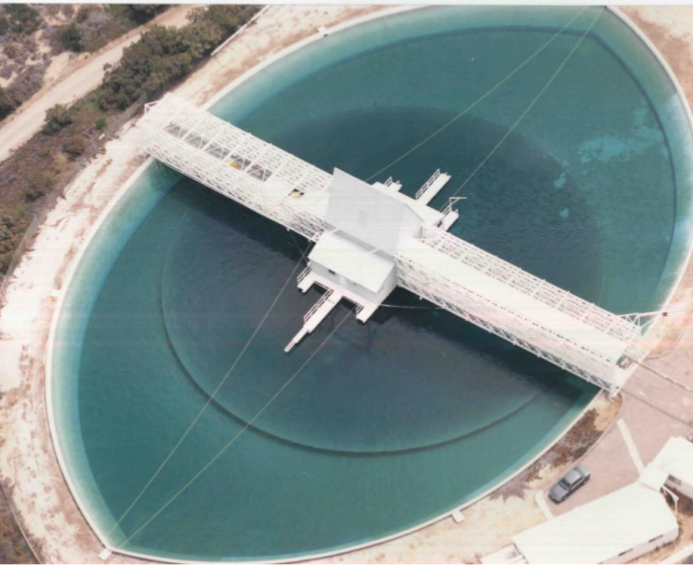
\includegraphics[width=0.8\textwidth, height=0.3\textheight]{transdec_aerial.png}
        \caption{Aerial view of TRANSDEC. Operational depth of 16 ft for most vision tasks}
        \label{fig:transdec_aerial}

\end{figure}

\subsection{Description of vision tasks}
Vision tasks in Robosub can divided into forward-facing tasks and bottom-facing tasks which poses different sets of challenges. Since the tasks do not vary significantly every year, we can use datasets collected from this year's competition as testbed for our vision algorithms.

\begin{figure}[ht]
\centering

        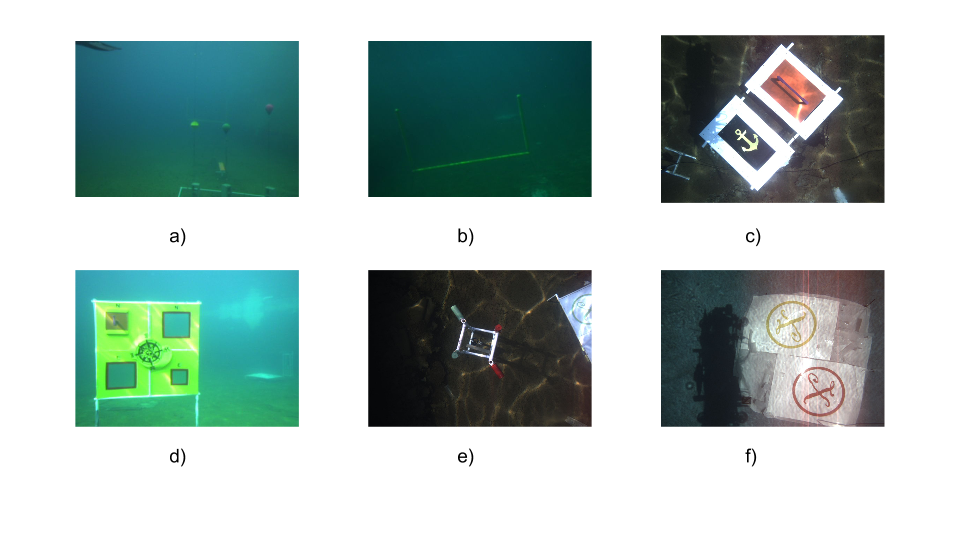
\includegraphics[width=0.8\textwidth, height=0.3\textheight]{robosub_vision_tasks.png}
        \caption{Robosub 2016 Vision Tasks. a) Scuttle Ship b) Navigate Channel c) Weigh Anchor d) Set Course e) Bury Treasure (Coins) f) Bury Treasure (Island)}
        \label{fig:robosub2016_tasks}

\end{figure}

\begin{enumerate}
    \item \textbf{Scuttle Ship (Buoy)}
        A recurring task where the AUV has identify the correct color buoy and touch it. There are two major challenges with this task:
        \begin{enumerate}[labels=(\alph*)]
        \item Red buoy tends to exhibit color distortion as red wavelength attenuates the fastest \cite{Galdran2015}.
        \item Non-uniform illumination on top-half of buoys make it hard to distinguish the buoys.
        \end{enumerate}
    \item \textbf{Navigate Channel} \\
        The AUV is required to move in between and over the PVC pipes.
    \item \textbf{Weight Anchor} \\
        Classic object classification task where the AUV is required to drop a marker into the correct bin to obtain maximum points after removing the cover using a manipulator.
    \item \textbf{Set Course} \\
        Identification of covered square (orange panel) and remove it. Fire two markers over 2 smaller holes. As yellow and orange are really close on the colour spectrum, this forces us to use other visual cues such as edge for better detection.
    \item \textbf{Bury Treasure} \\
        For this task, one has to identify the small cylinders (red and green) and drop them onto their respective colored circles (on the Island). Identifying and distinguishing small objects afar (4 m) underwater is the biggest challenge in this task. Besides that, the dropped cylinders may potentially occlude the circles.
\end{enumerate}

\section{Challenges in Underwater Image Processing}

Many literature such as \outcite{M2016} that investigates various underwater image restoration methods cite haze formation which happens as light propagated from object undergoes attenuation and scattering causing image with low contrast. In addition, Beer-Lambert law \cite{gevers2012color} states relates attenuation of light to properties of water medium; therefore, light components with low wavelength; green and blue are not as easily absorbed compared to red wavelength. This causes underwater images tend to have greenish or bluish color cast.

\begin{figure}[ht]
\centering

        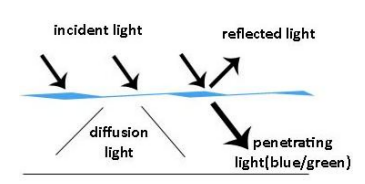
\includegraphics[width=0.8\textwidth, height=0.2\textheight]{underwater_beerlambert.png}
        \caption{Absorption of light at the surface}
        \label{fig:water_surface_effect}

\end{figure}

\section{Project Requirements Analysis}
Though it is the objective of the project to design a vision framework for the Robosub missions, the vision framework should also be easily extended to work for more complex real world applications. 

\subsection{Nature of tasks}
\begin{enumerate}
    \item Vision algorithms perform with acceptable accuracy under the following conditions:
    \begin{figure}[ht]
    \centering
            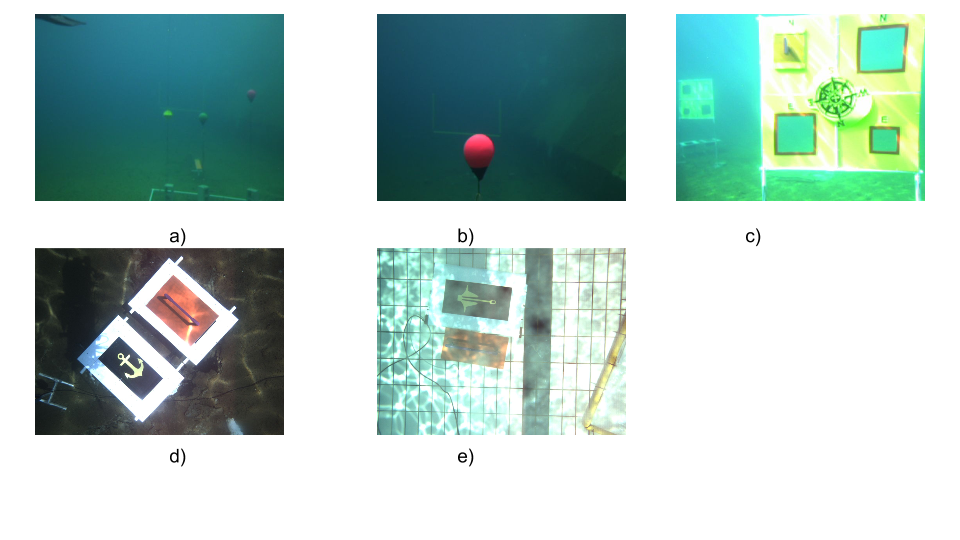
\includegraphics[width=0.8\textwidth, height=0.3\textheight]{task_challenges.png}
            \caption{Different vision challenges. a) Haze formation b) Partial occlusion c) Non-uniform illumination d) Sunlight flickers e) Shadow}
            \label{fig:vision_challenges}
    \end{figure}
    \item Low detection latency (near real-time) \\
        AUV needs to make swift decision based on sensor inputs to complete task under time constraints (same for real world time critical mission i.e underwater mine detection)
    \item Geometric properties of objects are made known in advance
    \item Short-period single target tracking for  task (unlike video surveillance application)
    \item Able to detect objects from far away (5m) and near distance (for manipulation task)
\end{enumerate}

 
\chapter{Literature Review}
This review is conducted with the purpose to investigate and select most suitable algorithms that generate the best result on the Robosub datasets. Since every teams who participate in Robosub are required to submit a journal paper,vision algorithms deployed by top-peforming schools such as Cornell University, University of Florida and École de technologie supérieure provide valuable insights on image processing that are effective in underwater environment. Besides that, review of popular image processing techniques in particular on topics like object detection, object tracking, color constancy, saliency mechanism, detection proposals and adapatation of algorithms.

\section{Preprocessing}
\subsection{Underwater Image Enhancement}
The paper by \outcite{garcia2002way} compared methods such as homomorphic filtering and local adaptive histogram equalization (Contrast Limited Adaptive Histogram) which considers that image is a product of illumination and reflectance properties. However, homomorphic filter has the benefit of preserving sharp edges while attenuating non-uniform illumination. On the other hand, by only redistributing pixels exceeding a clipping level to increase contrast of an image, CLAHE manages to reduce noise amplification in normal local histogram equalization.

Instead of relying on a single image, \outcite{Gracias2008} recover corrupted underwater image by finding the difference between the current frame with temporal median of a registered set of N frames. Image dehazing is equally as important to ensure good performance of further image processing operation such feature detection. \outcite{Kaiming2011} proposed a single image dehazing method using the dark channel prior which states that haze-free image contains local region with low intensities in at least one color channel. \outcite{Galdran2015} propose a variant of dark channel prior for underwater environment, the Red Channel method as red color shows most degradation in turbid water medium. From another perspective, \outcite{Ancuti2011} takes a fusion-approach to recover the original image by generating a few weight maps that correlates with intrinsic properties of the image itself. A color corrected and contrast enhanced of the input image are used to generate different weight maps that are fused using a Laplacian multi-scale strategy to generate a smoothed output image. This method has the benefit of using a single image but the weight maps must be combined with different weightage to achieve an ideal result. 

\subsection{Color Constancy}
Color cue plays an important role to distinguish different objects such as the small cylinders in Robosub that requires sorting by color. The ability to account for color of the light source is called color constancy. The work of \outcite{Gijsenij2011} analyzes various color constancy algorithms. Attention is paid especially on low-level statistics methods that are computationally inexpensive compared to learning-based methods. The Grey-World \cite{buchsbaum1980spatial} estimate the color of the light source by estimating the average color in the image assuming that any deviation from average color (Grey) is caused by illuminants. The White-Patch method \cite{land1977retinex} estimates the color of light source by computing the maximum response in individual RGB color channels. \outcite{finlayson2004shades} shows that both Grey-World and White-Patch algorithms are special instantiation of a more general color constancy algorithm based on Minkowski norm called Shades of Grey. Their investigation of best illumination estimation suggests using Minkowski norm, p = 6 to obtain optimal performance.

Though we see new method such as the Color Rabbit \cite{Bani??2014} which combine multiple local illumination estimations to a global one, these class of methods are more computationally expensive which is not suitable for real-time application. Inspired by primary visual cortex (V1) of human visual system (HVS), \outcite{Gao2013} estimate the true illuminant color of a scene by computing the maximum response in separate RGB channels of the responses of double-opponent cells. This method is shown to perform better on outdoor scenes from Gehler-Shi dataset where the mean reflectance is not achromatic which is assumed by Grey-World based methods. 

\section{Saliency Region Detection}
Ability of human visual system (HVS) to selectively process only the salient visual stimuli, specifically salient object detection helps to reduce computation time of object recognition that traditionally relies of sliding-window approach to detect object of interest. \outcite{achanta2009frequency} estimate centre-surround contrast using color and luminance features using a frequency-tuned approach to generate high-resolution saliency map. In contrast, biological inspired method of \cite{Itti1998} that computes centre-surround contrast using Difference of Gaussian (DoG) which generates low resolution map and ill-defined boundaries because of down sampling of original image.Because saliency detection often work poorly in low contrast environment i.e underwater environment, work of \outcite{VanDeWeijer2005} boost local color information by analyzing isosalient colour derivatives. \outcite{Cao2010} extended work of Van de Weijer as Gaussian derivatives of each opponent color to get a better iso-salient transformation. 

\section{Detection Proposals}
Relying on saliency mechanism is insufficient in perturbed underwater condition; therefore, different detection proposals algorithms are investigated. \outcite{Hosang2015} cited that "detection proposals" which can be grouped into a) grouping proposal methods and b) Window scoring proposals methods are used extensively by top performing object detectors in PASCAL and ImageNet. On top of reduced computation cost by avoiding exhaustive sliding window approach, detection proposals improve recall by filtering out false positives. Recent work of \outcite{Winschel2016} combines top performing detection proposals methods, SelectiveSearch \cite{uijlings2013selective} and EdgeBox \cite{zitnick2014edge}. Though detection proposals allow for faster object recognition, it is important that it does not filter out object of interest and incur more computation costs that out weights time saved.

\section{Object Detection and Tracking}
An overall review of journal papers submitted by top-performing teams in Robosub shows a general trend of combining surprisingly simple computer vision techniques such as adaptive color thresholding, edge detection i.e Canny Edge \cite{canny1986computational}, and contour analysis i.e Hu moment \cite{hu1962visual}. Team CUAUV (Cornell AUV) proposes adaptive color thresholding on different color spaces such as LAB, LUV and YCrCb where the individual masks are combined to form final binarized mask. This is a blob-based detection approach where contour generated by OpenCV's implementation of  \cite{suzuki1985topological}  will be matched against known geometric properties of desired object of interest. \outcite{Walters2014} use particle filter approach to detect and track object of interest. Known for its ability to deal with non-linear noise and multi-modal hypotheses \cite{isard1998condensation}, particle filter has the ability to recover from wrongly tracked objects. Though more sophisticated techniques such as neural-network classification is deployed, teams still generally rely on low-level visual cues such as color and edge. This may be attributed to simplicity and efficiency of mentioned algorithms. \outcite{Benoit2014} 
focuses on developing sophisticated vision tuning client that allows for rapid prototyping via "mix and match" approach to design a suitable vision pipeline for each individual vision tasks.

\chapter{Design \& Implementation}
\section{Vision Architecture}
    \begin{figure}[ht]
    \centering
            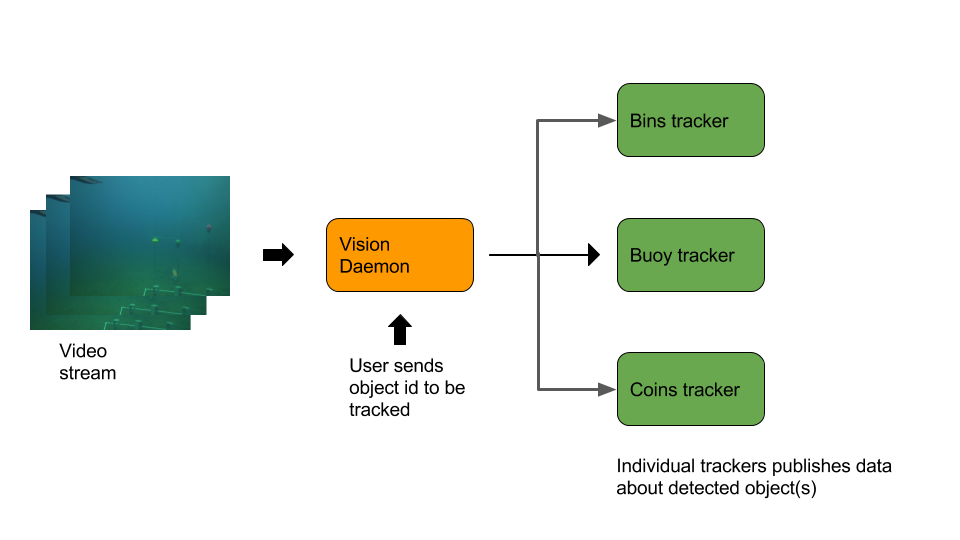
\includegraphics[width=0.8\textwidth, height=0.3\textheight]{overall_vision_architecture.png}
            \caption{BBAUV Vision Architecture}
            \label{fig:vision_architecture}
    \end{figure}
    
Our vision framework is implemented as a vision daemon running in the background when the AUV is launched. The vision framework is  integrated with ROS (Robotics Operating System) \cite{quigley2009ros}, an open source meta-operating systems used widely in robotics which provides message interface for inter-process communication (IPC). The vision daemon will initialized a new tracker upon request from the user (if the object is not currently being tracked). One advantage of this approach allows for parallel development of vision algorithms before competition which not speed up development but resulting in modular vision algorithms that are substitutable. 
\section{Methodology}
Individual object trackers are implemented using a tracking-by-detection approach where theese trackers had already been implemented and deployed in Robosub 2016. Below shows the vision pipeline of the baseline object tracker:
    \begin{figure}[ht]
    \centering
            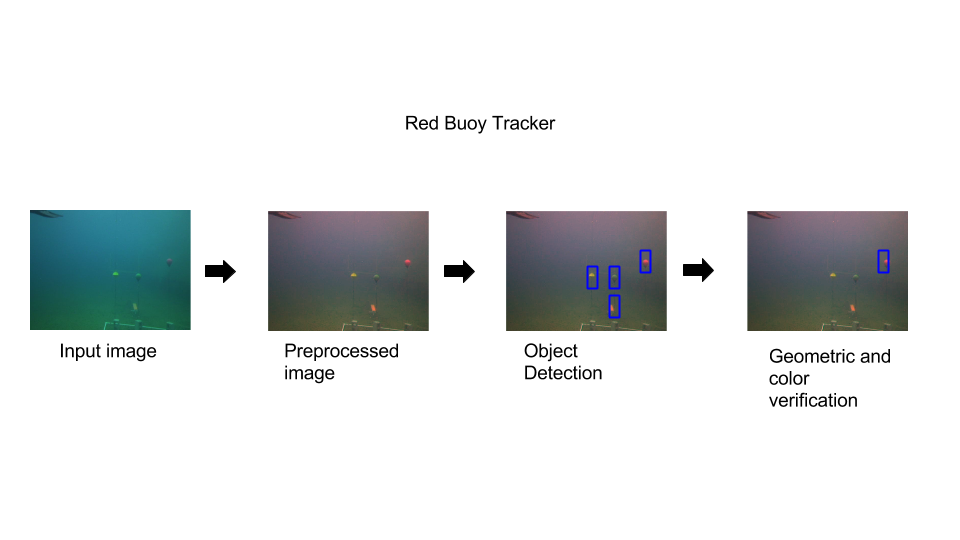
\includegraphics[width=0.8\textwidth, height=0.3\textheight]{object_tracking_pipeline.png}
            \caption{Object Tracking Pipeline}
            \label{fig:object_tracking_pipeline}
    \end{figure}
    
\subsection{Preprocessing} 
Input image first undergoes preprocessing before being processed by individual object detector. A design decision has been made to perform preprocessing on demand to a) reduce computation cost and b) customize preprocessing for different type of vision tasks. From past experiences, objects with distinct color from environment and bottom-facing objects can be detected without much preprocessing. Preprocessing can be separated into color constancy algorithms and underwater image enhancement algorithms. 

\subsubsection{Implemented Color Constancy Algorithms}
    \begin{figure}[h]
    \centering
            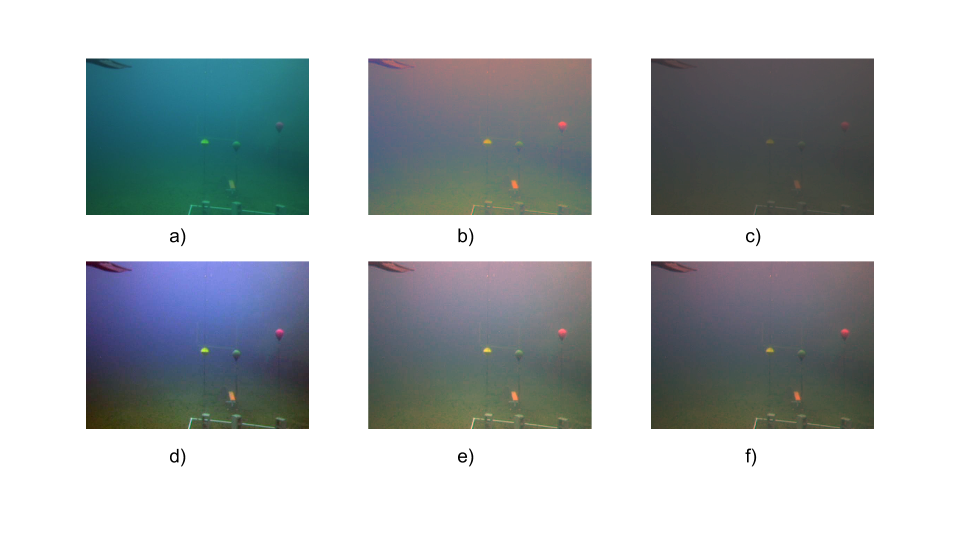
\includegraphics[width=0.8\textwidth, height=0.3\textheight]{color_constancy.png}
            \caption{Color constancy algorithms a) Original image b) Finlayson's comprehensive normalization c) Grey world d) Image Adaptive Contrast Enhancement (IACE) e) Non-iterative normalization f) Shade of Grey }
            \label{fig:color_constancy}
    \end{figure}
Various color constancy yields different results based on different underwater conditions. We can observe that some color constancy algorithms produce image with red hue which may affect performance of color-based object detectors. It must be known that gamma correction is performed after performing Grey-World algorithm to produce image with sufficient lighting. \outcite{Gijsenij2011} suggests that several approaches are combined to achieve optimal result. 

\subsubsection{Underwater Image Enhancement}
    \begin{enumerate}
        \item Gamma correction \\ To reduce effect of overexposure or underexposure because of camera settings. Sudden change in illumination because of cloud movement or position of the sun can be catastrophic.
        \item Homomorphic filter \\ To reduce flickering effect of bottom- facing tasks. This is implemented on the spatial domain \cite{nnolim2008homomorphic}
    \end{enumerate}
    
\section{Saliency Region Detection}
\begin{figure}[h]
    \centering
            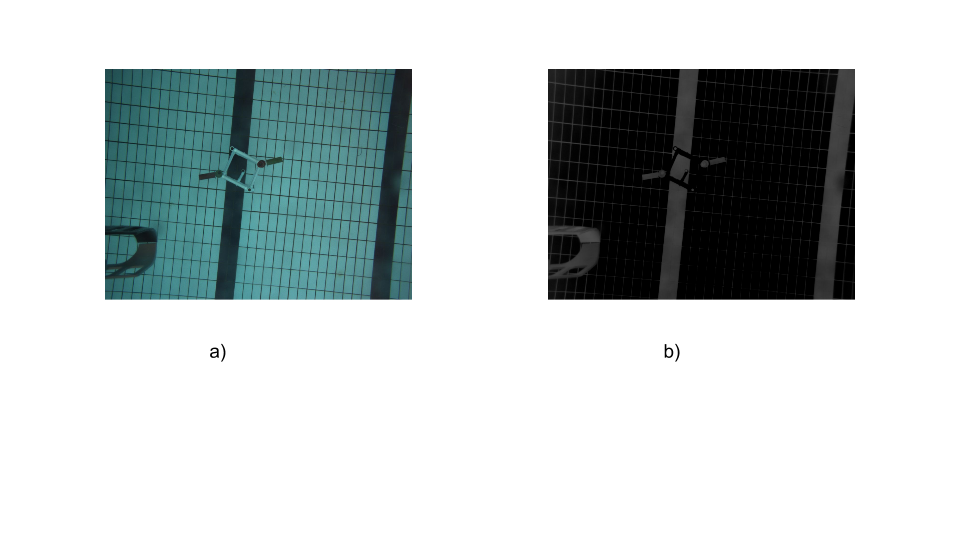
\includegraphics[width=0.8\textwidth, height=0.3\textheight]{saliency.png}
            \caption{Salient object detection of cylinders a) original image where color of cylinders severely degraded b) saliency map still mangages to capture the cylinders}
            \label{fig:saliency_detection}
    \end{figure}
The saliency detection approach of \cite{achanta2009frequency} is implemented to detect salient objects underwater as competition obstacles are often more salient than other features. Experiments have shown that images needed to be contrast enhanced and color corrected to achieve reliable detection. 

\chapter{Plan for the next semester}
\section{Implement more robust object detection and object tracking algorithms}

\subsection{Improve object detection}
Moving on, achieving consistent and accurate detection of objects in more difficult environments such as partial occlusion, sudden illumination change and presence of shadow. Taking inspirations from success of top object detector such as \outcite{Yang2014} that aggregate multiple-channel features; a multi-cues approach that includes both global and local features will be implemented to increase robustness of current object detector.

\subsection{Better object tracking}
One limitation of current tracking approach is neglecting prior tracked position which can help to prevent drift and reduce false positives. Instead of traditional particle filter that ignores current measurement in its system model and use only color model for its observation model, the project look to integrate more features such as optical flow and salient features. 

\section{Automate parameters selection and model selection}
Unlike approach taken by other schools that rely on manual visual tuning to achieve robust object tracking, the project aims to take inspirations from works of \cite{Zhang2016} and \cite{collins2005online} that attempt to map algorithms-parameters pair to specific dataset. A similarity function is then used to measure difference between test images with trained images.

\section{Experimental Setup}
In order to perform evaluation on proposed vision framework, several performance metrics will be used but the project adopts approach of \outcite{Luo2014} that uses: a) MOTA (Multiple Object Tracking Accuracy) b) MOTP (Multiple Object Tracking Precision) Average Overlap (Intersection-over-Union of bounding box). 

\subsection{Real-world dataset}
Recorded images from Robosub 2015, Robosub 2016 and Queenstown Pooltest will be labelled and used to evaluate performance of proposed vision algorithms. These datasets will be divided according to different challenges such as buoy detection, bins detection and coins detection.

\section{Proposed Time-line}
\begin{center}
    \begin{tabular}{ | l | p{10cm} |}
    \hline
    Time Period & Work to be done \\ \hline
    December Holiday & Propose and implement a set of object detection and object tracking that will work in different underwater conditions
    \\ \hline
    January & Validate proposed approach by comparing their performance with the baseline.
    Identify ways to automate parameter selection and model selection based for different tasks or scenarios
     \\ \hline
    February, March, April & Report writing on experimental results and findings
    \\
    \hline
    \end{tabular}
\end{center}

\bibliographystyle{socreport}
\bibliography{fyp}{}

%%% End document
\end{document}